\documentclass{njubachelor}

\sid{141220122} %学号
\grade{14} %年级

\cauthor{徐志航} %学生姓名
\ctitle{多风格的语音合成系统} %题目
\cdepartment{计算机科学与技术系} %院系
\cspecialization{计算机科学} %专业
\cmentor{俞凯}{教授} %指导老师 职称
\ckeywords{} %关键词
\cdate{} %提交日期

\eauthor{} %UNDERGRADUATE
\etitle{} %THESIS
\edepartment{} %DEPARTMENT
\especialization{} %SPECIALIZATION
\ementor{}{} %MENTOR MENTORTITLE
\ekeywords{} %KEY WORDS

\begin{document}

\makectitlepage

\begin{cabstract}
中文摘要。
\end{cabstract}

\begin{eabstract}
English abstract.
\end{eabstract}

\pagenumbering{Roman}
\thispagestyle{plain} %该页一般无页眉
\vspace*{0em}
\maketoc

\newpage
\pagenumbering{arabic}

\thispagestyle{plain} %该页一般无页眉
%\makectitle


\section{绪论}

\subsection{人工智能}
人工只能是计算机科学领域长期的研究方向之一。


\subsection{语音合成}

\subsection{基于隐马尔科夫模型的统计参数语音合成}

\subsection{本文组织结构}



\section{隐马尔科夫模型}
隐马尔科夫模型(Hidden Markov Model, HMM)是一种在许多领域被广泛使用的统计学时序模型,尤其是在语音识别和合成领域。

\subsection{定义}
隐马尔科夫模型是一个产生离散时间观察序列的有穷状态机。在每一个时间单元,隐马尔科夫模型通过状态转移概率改变状态,通过输出概率产生当前状态的观测数据。一个N-状态的HMM的参数我们记为 $$ \lambda = (A,B,\pi) $$
\begin{itemize}
	\item 状态转移概率
	\item 输出概率
	\item 观测序列
	\item 状态序列
	\item 状态时长
\end{itemize}

\begin{figure}
	\centering
	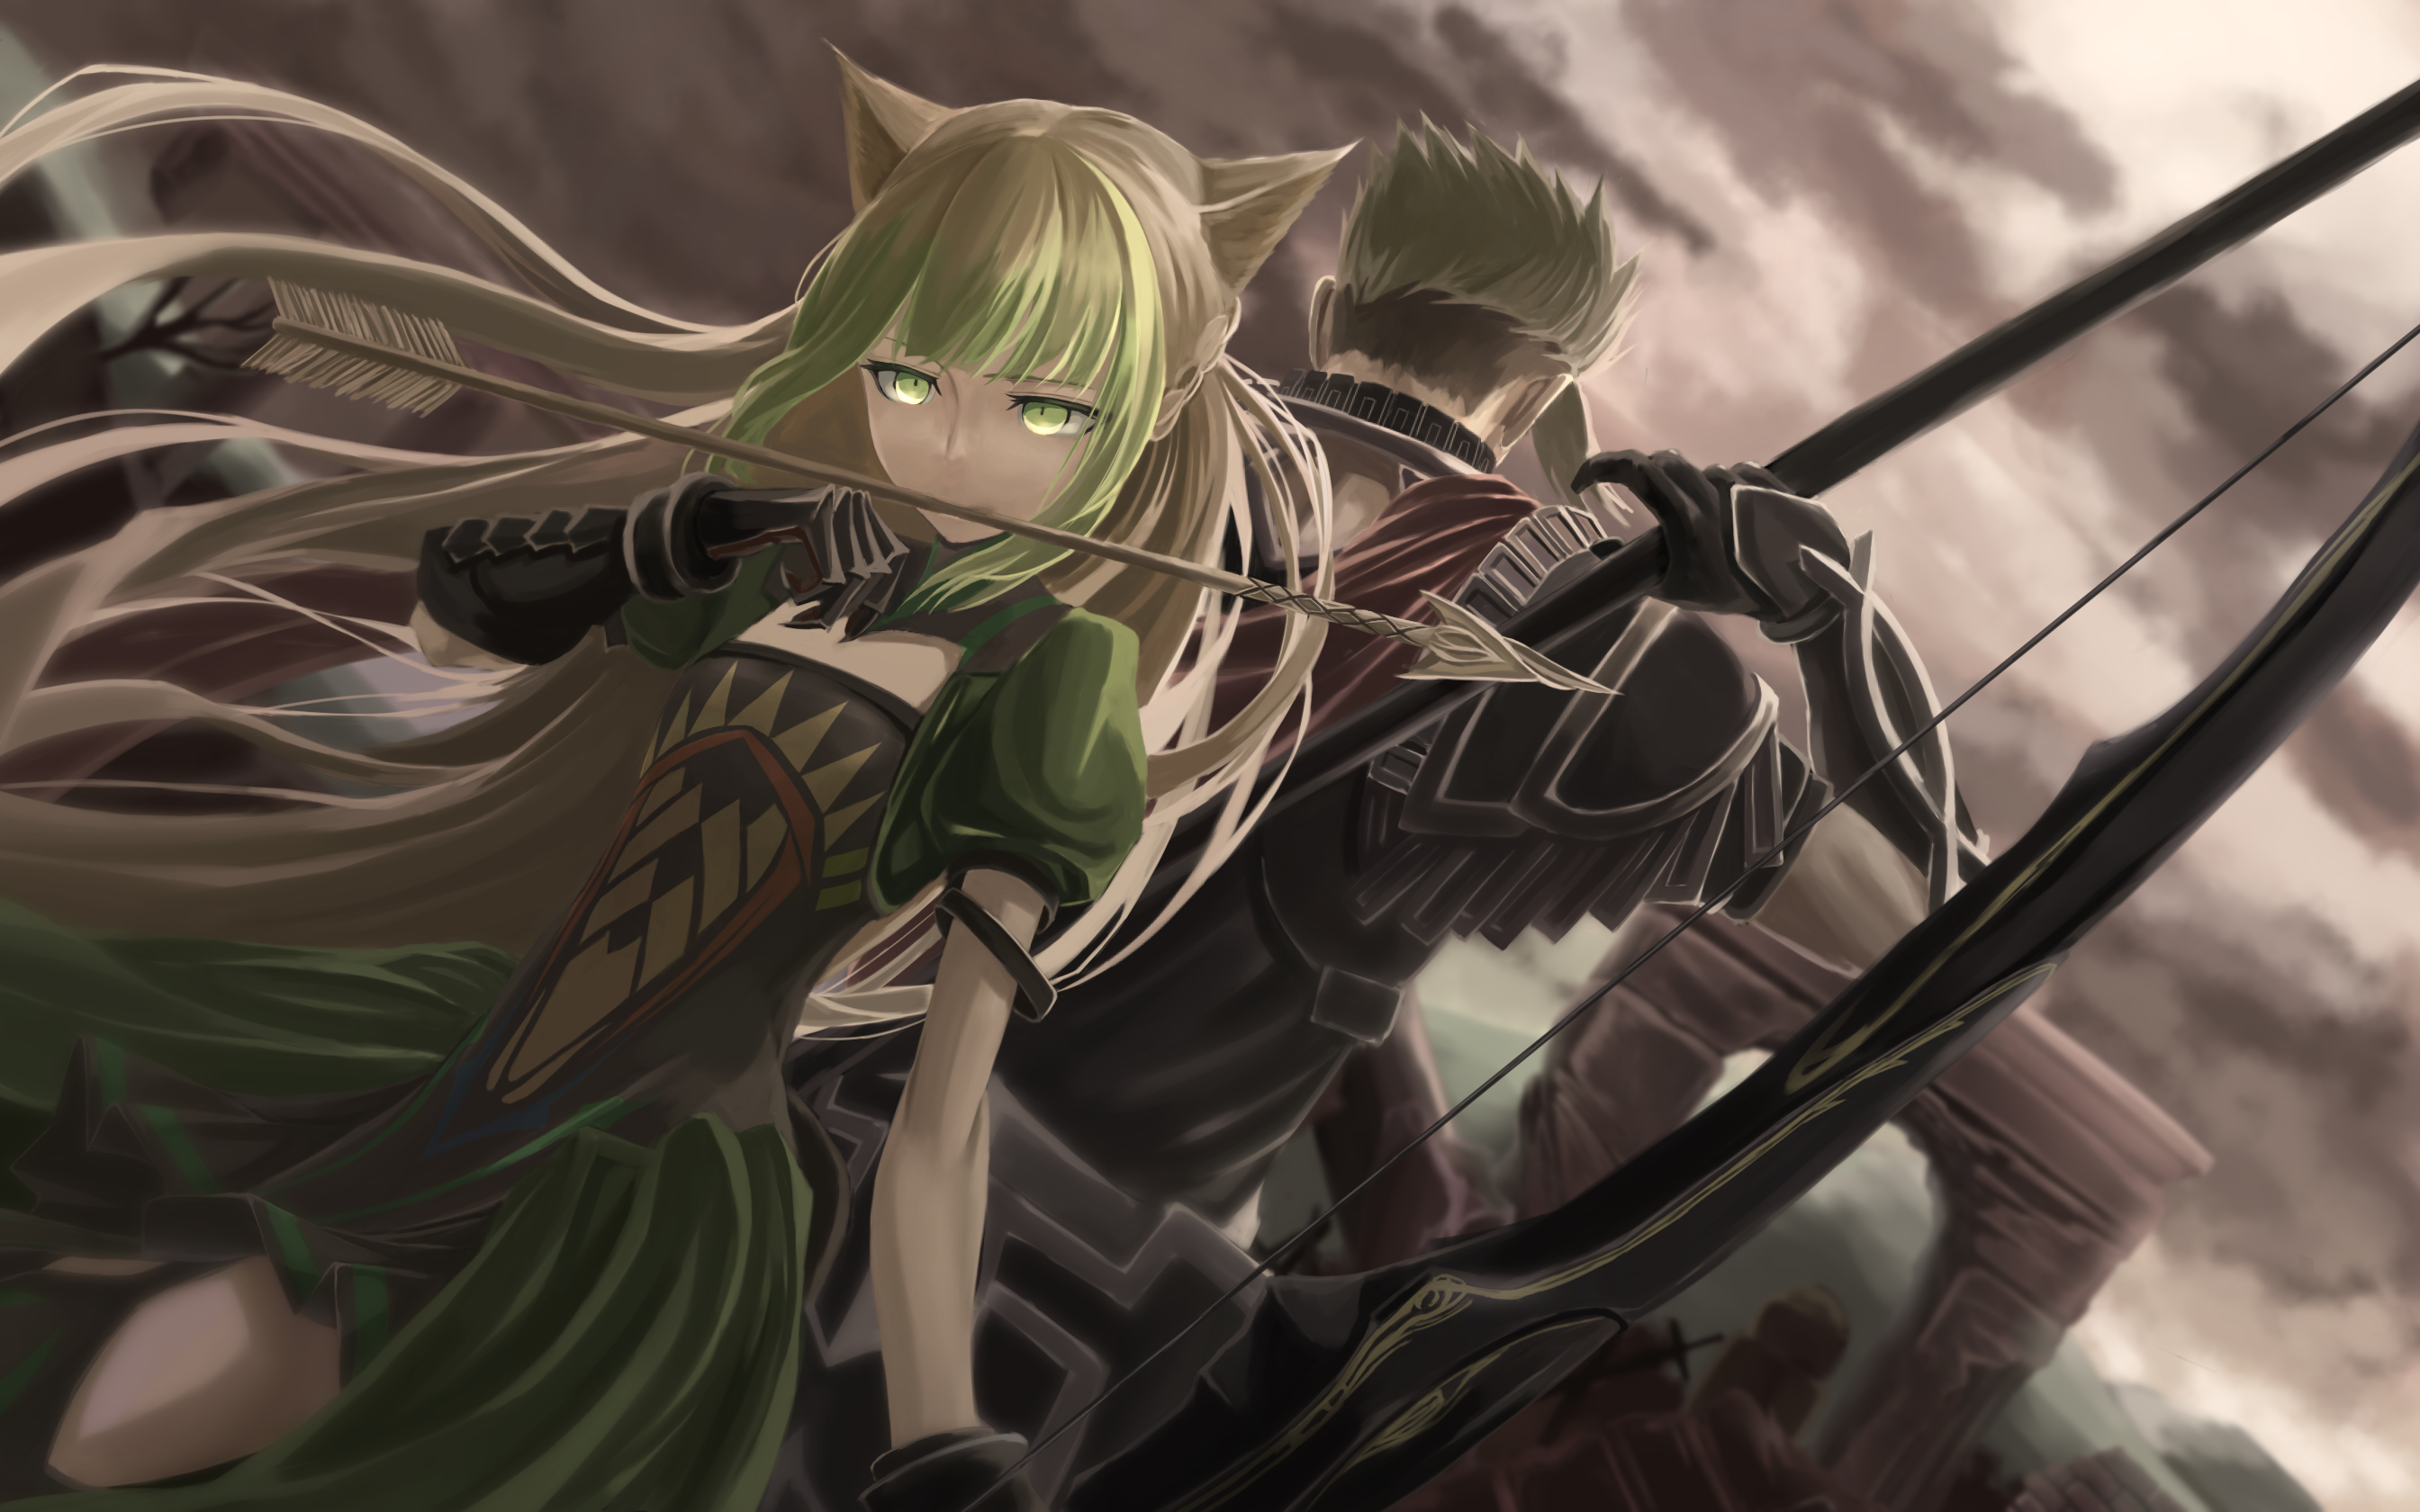
\includegraphics[width=.8\textwidth]{figures/test.jpg}
	\caption{这个是状态说明示例图}
\end{figure}
\subsection{最优状态序列}
大概是写先验概率 $$ P(O|\lambda)=\sum_{q}{P(O,q|\lambda)} = \max_{q}{P(O,q|\lambda)}$$
的计算,前向后向算法,viterbi解码
这个看<<统计参数学习>>比较清楚
\subsection{参数估计}

\section{基于隐马尔科夫模型的语音合成}
\subsection{参数生成算法}
\subsection{多空间概率分布}	% 可能不需要	
\subsection{决策树上下文聚类} % 可能不需要
\section{说话人自适应}
\subsection{MLLR 适应}
\subsection{Tying Transformation Matrices}
\section{Speaker Adaptive Trainng}
\subsection{Average Voice Model Training}
\section{说话人混搭}

主体

\subsection{第二节~第一小节}

主体 1

\subsection{第二节~第二小节}

主体 2


\newpage
\pagenumbering{Roman}

\begin{thebibliography}{99}
\bibitem{citekey1} 参考文献条目一.
\end{thebibliography}

\newpage
\ack

致谢内容

\newpage
\appendix

\section{附录一}

\subsection{附录 1.1}

附录内容

\end{document}
